\documentclass[11pt]{article}
\usepackage[margin=0.6in]{geometry}
\usepackage[utf8]{inputenc}
\usepackage{authblk}
\usepackage{doi}
\usepackage{tcolorbox}
\usepackage{enumitem}
\usepackage{graphicx,pdflscape,multirow}
\usepackage{array}
\usepackage{xcolor}
\usepackage{multicol}
\usepackage{wrapfig,lipsum,booktabs}
\usepackage{fancybox}
\usepackage{amsmath}

\newcommand{\fixme}[1]{{\color{red} (#1)}}
\newcommand{\coloc}{\texttt{escheR}}

% \renewcommand\Authfont{\fontsize{8}{14.4}\selectfont} % change author fontsize
% \renewcommand\Affilfont{\fontsize{6}{10.8}\itshape}   % change auth affil fontsize
\makeatletter % make affiliations on one line
\renewcommand\AB@affilsepx{, \protect\Affilfont}
\makeatother

\usepackage[sort&compress,square,numbers]{natbib}
\bibliographystyle{unsrtnat}

%\setmainfont{Helvetica}
\title{\coloc: Optimize Spatial Visualization Following Gestalt Principles}
\author[1]{Boyi Guo\thanks{Corresponding author}}
\author[1]{Stephanie C. Hicks}
\affil[1]{Department of Biostatistics, Johns Hopkins Bloomberg School of Public Health, MD, USA}
\date{\today}

\begin{document}
\maketitle

\vspace{-.6in}

%% ABSTRACT ============================================================================================
\section*{Abstract}
\subsection*{Summary}
Visualization is an indispensable component of data analysis and receives growing recognition as essential. Nevertheless, current methods and
tools are inadequate to visualize the novel spatially-resolved data, limiting the ability to derive new insights and discoveries. Specifically, there are no multi-dimensional \textit{in-situ} visualization that simultaneously displays multiple variables in a 2D spatial map. To address this problem, we introduce gestalt principles to the design of spatial maps, layering aesthetics to display multiple variables. The proposed visualization can be broadly applied to spatially resolved data and 2D embedding methods. We provide an open-source R package \coloc, which seamlessly integrates into the state-of-the-art spatial omics toolboxes.

\subsection*{Availability and implementation}
The R package \coloc is freely available at Github (\url{https://github.com/boyiguo1/escheR}).
% and Zenodo (\fixme{add link}).


%% INTRODUCTION ============================================================================================
\section*{Introduction}
Visualization is an indispensable component of data analysis, providing clarity that connects quantitative evidence to key conclusions.\cite{dagostinomcgowan_2022} In bioinformatics research, visualization receives growing recognition as essential: many scientists rely on visualization to complete their cognitive process from analysis to insight, including analytic validation of automated pipelines and scientific communication.\cite{odonoghue_2021} Nevertheless, current methods and tools are inadequate to visualize the growingly complex biological data and computational models, limiting the ability to derive new insights and discoveries.\cite{odonoghue_2010}  

The recent technology breakthrough in spatial profiling enables characterizing the diversity of molecules, e.g. DNA, RNA, and proteins, in the spatial context\cite{moffitt_2022}, generating novel spatially-resolved data that requires highly tailored \textit{in situ} visualizations\cite{dries_2021, Lewis_2021, odonoghue_2021}. Current \textit{in situ} visualizations, as opposed to embedding visualizations (e.g. t-SNE \cite{hinton_2002} and UMAP \cite{becht_2019}) that project information to some mathematical space, visualize molecular information in the original cellular location, creating spatial maps that color-code a single variable (e.g., molecule expression, cell type, or spatial domain). This approach lacks the ability to simultaneously exhibit multiple variables, possibly from disparate data domains (such as expression domain and spatial domain) or modalities (such as transcriptomics and proteomics), creating cognitive gaps to interpret findings regarding their (micro-) environment. For example, when studying differential expression in different spatial domains (commonly defined by tissue architecture, e.g. cancerous regions, cortical layers), two spatial maps are displayed side-by-side, one for gene expression and one for spatial domains, creating significant challenges to associate these two information together. While software-based interactive visualizations\cite{sriworarat_2023} or 3-D visualizations have the potential to mitigate this challenge, they are infeasible for scientific communications in static media, such as prints. Developing a static spatial visualization that enables the simultaneous display of multiple dimensions of information is crucial for spatially-resolved data research.


% Previous data visualization of omics largely relies on projecting the omics space to an embedding space, such as t-SNE and UMAP, which is infeasible for spatial omics technologies.

 To optimize \textit{in situ} visualization, we introduce gestalt principles to the design of spatial maps. Gestalt principles\cite{todorovic_2008, palmer_1999} refer to a set of rules describing how humans perceive and interpret visual information and are commonly applied in art and designs. Following gestalt principles, we add additional visual dimensions to spatial maps, leveraging different aesthetics, such as color, fill, and symbols, to simultaneously display disparate variables. Specifically, we apply figure-ground articulation to display two variables: one variable (e.g. expression) can be plotted as color-filled circles, serving as the \textit{figure}; one variable (e.g. spatial domains) can be plotted as the backgrounds of the circles, creating a \textit{ground} for the figure. For adjacent circles with limited space between them to display the background color, we use an economic implementation, colored outlines for these circles, inspired by watercolor effect\cite{pinna_1987, pinna_2001}. Watercolor effect describes the phenomenon in visual perception that surface color arises from thin boundaries and hence is applied here to perceive the background color in tight space. Overall, the figure-ground articulation creates two isolated layers in visual perception to display the two variables while maintaining the relative spatial relationship serving as a reference between the two. In addition, other fundamental principles\cite{todorovic_2008}, such as proximity, similarity, continuity, and closure, incentivize the brain to group elements and dimensions in the visualization, guaranteeing an integrative perception of the complex multi-dimensional spatial map.
 

To implement the proposed visualization, we leverage the state-of-art data visualization framework \texttt{ggplot2}\cite{ggplot2} following the grammar of graphics\cite{wilkinson_2012}. Specifically, we use an interactive process to layer each variable in spatial maps using different aesthetics. For example, we use the combination of \texttt{color} and \texttt{fill="transparent"} to create the background layer and \texttt{fill} to create the figure layer. When necessary to display an additional layer for a third variable, \texttt{shape} can be used to add symbols such as cross (+) and asterisk (*) to highlight in the spatial map. We provide an open-source package called \coloc (named after the graphic artist M.C. Escher) in the R programming environment\cite{R}, providing a simplified interface to navigate the implementation of the multi-dimensional \textit{in situ} visualization. By adapting \texttt{ggplot2} standard, \coloc can be seamlessly integrated into many popular spatial resolved toolboxes, such as \texttt{SpatialLIBD}\cite{pardo_2022}, \texttt{Seurat}\cite{hao_2021}, \texttt{Giotto}\cite{dries_2021} to name a few, and allow further theme customization with ease. We provide two use cases to exemplify some utility of the proposed spatial visualization: 1) the spatially differential gene colocalization in the human dorsolateral prefrontal cortex (DLPFC) using spatial transcriptomics data\cite{huukimyers_2023}; 2) multi-dimensional UMAP highlighting differential gene expression in data-driven cell clusters \cite{freytag_2020}. 

\section*{Use Case 1: Spatially Differential Colocalization in DLPFC}
In a recent study investigating the molecular organization of human dorsolateral prefrontal cortex (DLPFC) \cite{huukimyers_2023}, two schizophrenia risk genes, membrane-bound ligand ephrin A5 (\textit{EFNA5}) and ephrin type-A receptor 5 (\textit{EPHA5}), are identified to colocalize via the cell-cell communication analysis. In addition, data suggest Layer 6 is the most highly co-localized layer compared to other cortex layers. To visually examine the inference, we apply \coloc to create a multi-dimensional \textit{in-situ} spatial map (Figure \label{fig:visual}) that simultaneously exhibits the cortex layers (displayed with color-coded spot outlines) and the categorized colocalization status of \textit{FYN} and \textit{EFNA5} (displayed with color-coded spot fill). Compared to the traditional visualization where the cortex layers and the colocalization status are ploted in two side-by-side figures, our proposed visualization enables directly mapping colocalization status to the spatial domain, simplifying the perception of two sources of information and allowing cognitive comparison across cortex layers. 

\section*{Use Case 2: Multi-dimensional UMAP}
The application of the proposed framework doesn't limit to in-situ visualizations of spatially resolved data. It can be broadly applied to data mapped to any 2-dimensional coordinate system to simultaneously display multiple variables. Such systems include euclidean space (including spatial coordinate as a special case) and data-driven embedding space, for example, UMAP and t-SNE. To demonstrate, we apply the proposed visualization to address the challenge of simultaneously displaying cluster membership and gene expression in a single-cell UMAP plot. To address the overplotting problem, \texttt{schex} proposed to apply hexagonal binning strategy to unbiasedly display the gene expression.\cite{freytag_2020} In addition, color-coded convex hulls were used to annotate different clusters of cells (Figure \label{fig:visual}). Nevertheless, the convex hulls create substantial overlapping areas, creating confusion when interpreting cluster memberships of hexagons in the overlapping areas. To improve the interpretability of the visualization, we integrate the proposed visualization to \texttt{schex} by replacing convex hulls with color-coded hexagons boundaries  (Figure \label{fig:visual}) to avoid possible membership confusion. The visual improvement is easily implemented without any modification of \texttt{schex} thanks to the Grammar of Graphics \cite{wilkinson_2012} standard.

\vspace{0.45in}
In summary, we propose an innovative multi-dimensional spatial visualization to simultaneously display multiple variables in a 2D coordinate system. Specifically, our design leverages the gestalt principle from visual perception to introduce other dimensions of a spatial map by iterative layering aesthetics. Developed upon \texttt{ggplot2}, we provide an open-source R package \coloc that is seamlessly compatible with popular spatial resolved data analysis toolboxes. The proposed visualization has broad applications in visualizing both spot-based and image-based spatial resolved data, spatial multi-omics as well as other spatial-based data. The proposed visualization innovation highlights the importance and potential of translating theories in vision science to data science, addressing long-standing challenges in bioinformatics data visualization.


% While \coloc is to design to display colocalization in their spatial context, the underlying principle can be broadly applied to address visualizaiton challenges in informaiton rich visualizations. The contrast color optical illusion provides allows to add another dimension of information in any spatial visualization, which can be further used to display multi-omics presence, greatly improve the interpretability. 

% our programming provides flexibility by following the grammar of graphs, especially ggplot2




%% EPILOGUE ================================================================
\section*{Acknowledgements}
B.G. would like to acknowledge Dr. Leonardo Collado Torres, Louise Huuki-Myers and Leon Di Stefano for their helpful feedback.

\vspace{0.2in}
\noindent \textit{Conflict of Interest:} none declared.

\section*{Data availability}
The spatial transcriptomics dataset was obtained from \texttt{spatialLIBD} (\url{http://research.libd.org/spatialLIBD/}). The UMAP example follows the tutorial from \texttt{schex} (\url{https://www.bioconductor.org/packages/release/bioc/vignettes/schex/inst/doc/using_schex.html}). The code that generates these figures are deposited at \fixme{github manuscript repo}.

\clearpage
% \vspace{-0.1in}
\begin{wrapfigure}[13]{r}{0.8\textwidth}
\vspace{-0.3in}
\begin{center}
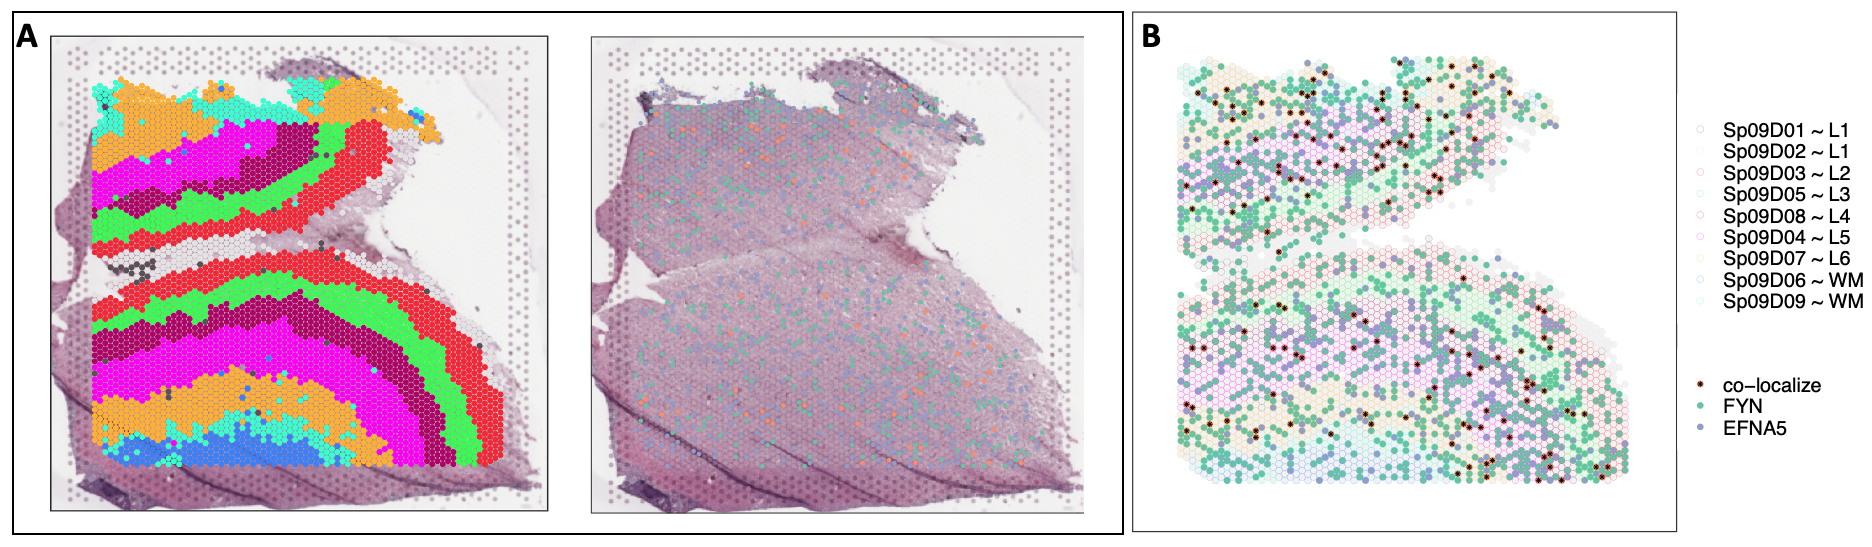
\includegraphics[width=0.78\textwidth]{figure/new_visiual.png}
\end{center}
\vspace{-0.35in}
\caption{\footnotesize \textbf{Optimized visualization interpreting co-localization in the spatial context}. (\textbf{A}) Current visualization of co-localization requires two separate plots, one to display spatial domain information and one to display co-localization, difficulty to associate the two sources of information for interpretation. (\textbf{B}) The proposed visualization is optimized to display both spatial domain and co-localization information in one plot.}
\label{fig:visual} 
\end{wrapfigure}

%% BIBLIOGRAPHY ==========================================================

\clearpage 
% \printbibliography
\bibliography{refs}

\end{document}


